\documentclass{article}
\usepackage[margin=1in]{geometry}
\usepackage{amsmath,amsfonts,amssymb}
\usepackage{listings}
\usepackage{color}
\usepackage{graphicx}
\usepackage{subfig}
\usepackage{blkarray}
\usepackage{multirow}
\usepackage{float}
\usepackage{caption}
\usepackage{subcaption}
\begin{document}
\begin{titlepage}
	\setlength{\parindent}{0pt}
	\large

\vspace*{-2cm}

\definecolor{dkgreen}{rgb}{0,0.6,0}
\definecolor{gray}{rgb}{0.5,0.5,0.5}
\definecolor{mauve}{rgb}{0.58,0,0.82}

\lstset{frame=tb,
  language=Python,
  aboveskip=3mm,
  belowskip=3mm,
  showstringspaces=false,
  columns=flexible,
  basicstyle={\small\ttfamily},
  numbers=none,
  numberstyle=\tiny\color{gray},
  keywordstyle=\color{blue},
  commentstyle=\color{dkgreen},
  stringstyle=\color{mauve},
  breaklines=true,
  breakatwhitespace=true,
  tabsize=3
}

University of Waterloo \par
CS 480 \par
\vspace{0.05cm}
r2knowle: 2023-09-20
\vspace{0.2cm}

{\huge Exercise \# 3 \par}
\hrule

\vspace{0.5cm}
\textbf{Q1)} To begin below is the code in python that was used to generate our results:

\begin{lstlisting}
import matplotlib.pyplot as plt
import numpy as np
import pandas as pd
from sklearn.linear_model import Ridge, Lasso, LinearRegression
from sklearn.metrics import mean_squared_error

# Estimates the best hyperparameter for ridge for a given dataset
def determineHyperParametersRidge(x, y):
    maxValue = 2000;
    hyper = 1;
    for h in range(1, 100):
        mse = []
        for i in range(0, 9):
            pos=len(x)/10
            train_x = x[0:i*pos] + x[(i+1)*pos]
            test_x = x[i*pos:(i+1)*pos]
            train_y = y[0:i * pos] + y[(i + 1) * pos]
            test_y = y[i * pos:(i + 1) * pos]
            ridge = Ridge(alpha=h/10)
            ridge.fit(train_x, train_y)
            pred_y = ridge.predict(test_x)
            mse.append(mean_squared_error(pred_y, test_y))
        if (maxValue > np.average(mse)):
            maxValue = np.average(mse)
            hyper = h
    print(maxValue)
    return hyper
# Estimates the best hyperparameter for lasso for a given dataset
def determineHyperParametersLasso(x, y):
    maxValue = 2000;
    hyper = 1;
    for h in range(1, 100):
        mse = []
        for i in range(0, 9):
            pos = len(x) / 10
            train_x = x[0:i * pos] + x[(i + 1) * pos]
            test_x = x[i * pos:(i + 1) * pos]
            train_y = y[0:i * pos] + y[(i + 1) * pos]
            test_y = y[i * pos:(i + 1) * pos]
            lasso = Lasso(alpha=h / 100)
            lasso.fit(train_x, train_y)
            pred_y = lasso.predict(test_x)
            mse.append(mean_squared_error(pred_y, test_y))

        if maxValue > np.average(mse):
            maxValue = np.average(mse)
            hyper = h
    print(maxValue)
    return hyper


dataset = ["A", "B", "C"]

for i in range(0, 3):
    # Found using the above functions
    BestRidge = [9.4, 89, 10]
    BestLasso = [0.01, 0.01, 9]

    X_train = pd.read_csv("dataset/X_train_" + dataset[i] + ".csv", header=None)
    Y_train = pd.read_csv("dataset/Y_train_" + dataset[i] + ".csv", header=None)

    X_test = pd.read_csv("dataset/X_test_" + dataset[i] + ".csv", header=None)
    Y_test = pd.read_csv("dataset/Y_test_" + dataset[i] + ".csv", header=None)
    # Create our Models
    lin = LinearRegression()
    rid = Ridge(alpha=BestRidge[i])
    las = Lasso(alpha=BestLasso[i])

    # Train our Models
    lin.fit(X_train, Y_train)
    rid.fit(X_train, Y_train)
    las.fit(X_train, Y_train)

    maxCoef = max(lin.coef_.max(), rid.coef_.max(), las.coef_.max())
    minCoef = min(lin.coef_.min(), rid.coef_.min(), las.coef_.min())

    numberOfBuckets = 50

    # Create our Buckets
    divisFactor = int(np.abs(maxCoef) + np.abs(minCoef)) / numberOfBuckets


    linPred = lin.predict(X_test)
    ridPred = rid.predict(X_test)
    lasPred = las.predict(X_train)

    print("======= DATA: ", dataset[i], "=======")
    print("Linear Error: ", mean_squared_error(linPred, Y_test))
    print("Rid Error: ", mean_squared_error(ridPred, Y_test))
    print("Las Error: ", mean_squared_error(lasPred, Y_test))

    binsToSort = []
    for x in range(0, numberOfBuckets):
        binsToSort.append(minCoef + x * divisFactor)
    print(binsToSort)
    plt.hist(lin.coef_.flatten(), bins=binsToSort, alpha=0.5, color="r", label="Linear Regression")
    plt.hist(rid.coef_.flatten(), bins=binsToSort, alpha=0.5, color="g", label="Ridge Regression (h =" + str(BestRidge[i]) + ")")
    plt.hist(las.coef_.flatten(), bins=binsToSort, alpha=0.5, color="b", label="Lasso Regression (h =" + str(BestLasso[i]) + ")")
    plt.legend()
    plt.xlabel('Coefficient Weight')
    plt.ylabel('Number of Observations')
    plt.title("Prediction Buckets for Dataset " + str(dataset[i]))
    plt.grid(True)
    plt.show()

\end{lstlisting} 
\newpage
From this we get the following graphs and MSEs for the datasets:
\begin{figure}[H]
\begin{minipage}[c]{0.9\linewidth}
\centering
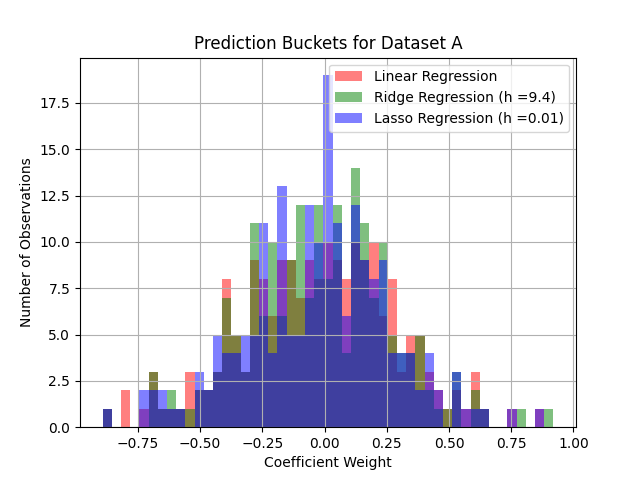
\includegraphics[scale=0.5]{3A.png}
\end{minipage}
\hfill
\vspace{0.5cm}
\begin{minipage}[c]{0.9\linewidth}
\centering
\begin{tabular}{ |c||c|c|c| } 
\hline
\text{ } & \text{Linear Regression} & \text{Ridge Regression} & \text{Lasso Regression}\\
\hline
\hline
\text{Mean Squared Error} & 3.2474 & 2.7828 & 21.1351 \\
\hline
\end{tabular}
\caption{Results for Dataset A}
\end{minipage}%
\hfill
\vspace{0.5cm}
\begin{minipage}[c]{0.9\linewidth}
\centering
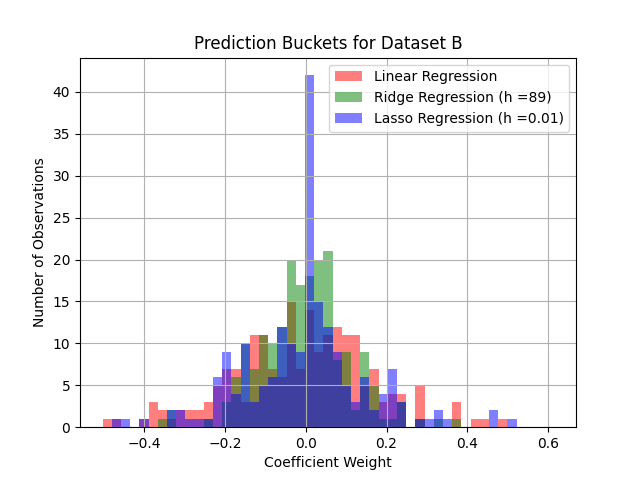
\includegraphics[scale=0.5]{3B.png}
\end{minipage}
\hfill
\vspace{0.5cm}
\begin{minipage}[c]{0.9\linewidth}
\centering
\begin{tabular}{ |c||c|c|c| } 
\hline
\text{ } & \text{Linear Regression} & \text{Ridge Regression} & \text{Lasso Regression}\\
\hline
\hline
\text{Mean Squared Error} & 2.7427 & 1.9097 & 5.5387 \\
\hline
\end{tabular}
\caption{Results for Dataset B}
\end{minipage}%
\end{figure} 

\begin{figure}[H]
\begin{minipage}[c]{0.9\linewidth}
\centering
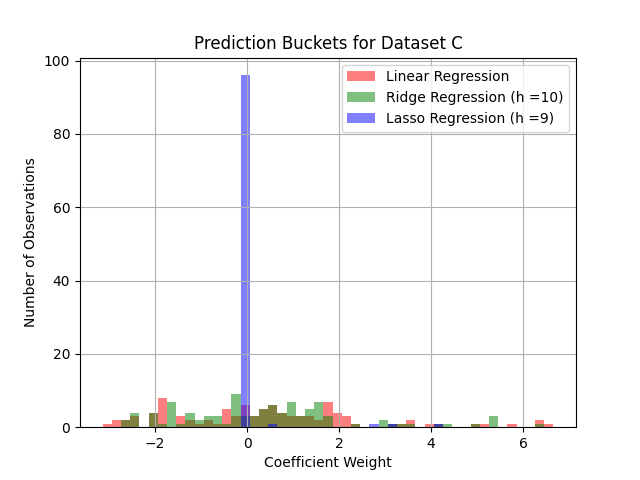
\includegraphics[scale=0.5]{3C.png}
\end{minipage}
\hfill
\vspace{0.5cm}
\begin{minipage}[c]{0.9\linewidth}
\centering
\begin{tabular}{ |c||c|c|c| } 
\hline
\text{ } & \text{Linear Regression} & \text{Ridge Regression} & \text{Lasso Regression}\\
\hline
\hline
\text{Mean Squared Error} & 502.35 & 514.83 & 1223.6 \\
\hline
\end{tabular}
\caption{Results for Dataset A}
\end{minipage}%
\end{figure}
From this it is clear that Lasso Regression preforms by far the worst on all the datasets, even when its hyper paramaters where tuned. Linear regression seems to do better then ridge regression on dataset C possible due to the very low sample data. However ridge regression does the best on the other two datasets with the lowest MSEs out of all the different regression methods.
\end{titlepage}
\end{document}